\chapter{Efficient Markets}

These notes follow Robert J. Shiller's lecture on efficient markets in \emph{Financial Markets}, curated by LazyingArt LLC. We are not given the theory as a finished doctrine. We are first given a puzzle. If market prices absorb public information, and if the market therefore ought to beat any one of us, what are we to do with David Swensen's long record of success at Yale? The lecture answers this in stages: first by showing how performance statistics can mislead, then by reconstructing the history of the efficient-markets idea, and finally by contrasting technical analysis with the random-walk and mean-reverting views of prices. The verdict is deliberate and limited: efficient markets is a half-truth.

\section{Opening paradox: efficient markets and David Swensen}

Shiller begins with the slogan form of the efficient-markets hypothesis. Markets incorporate public information. Therefore, if we think we are smarter than the market, the market will usually prove otherwise. In classroom shorthand, the idea says: you cannot beat the market by acting on information that is already public.

\begin{definition}
In the working sense of this lecture, the efficient-markets hypothesis says that publicly available information is incorporated into market prices so rapidly that one should not expect to earn systematic excess returns by trading on that information after it has become public.
\end{definition}

This would already be a strong claim. But the lecture refuses to let the claim remain abstract. Swensen, who had just lectured to the class, is said to have beaten the market for decades, beginning in 1985, and not merely by a small amount. The point is not only that Yale's endowment did well. The point is that this performance had visible institutional consequences. Yale's financial strength supported policies such as need-blind admissions on an international scale. Thus the opening question is not merely statistical. It is practical and institutional.

\subsection{Question \& Answer}

The natural question is: if Swensen appears to beat the market for decades, is that skill, luck, or a problem with the theory?

Shiller does not answer this immediately. He first blocks the easy answers. A defender of efficient markets may say that if millions of managers try, one of them will look brilliant by luck alone. That possibility cannot be dismissed out of hand. But neither should we settle the matter by pointing only to raw return. We must ask what risks were taken, how those risks were measured, and in what kinds of markets the manager was operating. The lecture therefore moves from the paradox itself to the machinery of performance measurement.

\section{Sharpe ratios, hidden tails, and the temptation to game the statistics}

The first technical checkpoint is the Sharpe ratio. Shiller reminds us that a high return by itself proves very little. Any expected return can be raised by taking more risk. That was already implicit in the efficient frontier and the tangency-line discussion earlier in the course. A proper performance measure must therefore scale return by risk.

In the classroom language of this lecture, one may write the Sharpe ratio cautiously as
\begin{equation}
S \approx \frac{E[R_p - R_b]}{\sigma(R_p)},
\end{equation}
where \(R_p\) is the portfolio return and \(R_b\) is a benchmark return. In the lecture, the benchmark is spoken of loosely as ``the market,'' so we keep the notation slightly generic while retaining the intended meaning.

The basic inputs are the mean and the standard deviation of return:
\begin{equation}
\mu_R = E[R], \qquad \sigma_R = \operatorname{SD}(R).
\end{equation}
If a portfolio has a high excess return but also a high standard deviation, the large return may simply be compensation for risk. In that sense the Sharpe ratio is supposed to correct the naive reading of performance.

Swensen's objection, as Shiller reconstructs it, is that for broad and illiquid portfolios the standard deviation may not be well measured at all. Private equity is not continuously traded. Real estate may sit for long periods with only appraisals rather than transaction prices. Appraisal-based valuations smooth the observed return series. The measured \(\sigma(R_p)\) can then be artificially low. Even before any trickery, the denominator is already suspect.

\begin{figure}
\centering

\includegraphics[width=0.74\textwidth]{lecture_07_figure_02.png}
\caption{The chalkboard bell-curve sketch used to introduce the return distribution. The axis label is only partly legible, but the safest reading is a horizontal return axis.}
\end{figure}

At this point Shiller sharpens the argument. Suppose a manager knows that outside investors are evaluating him by Sharpe ratio and suppose, further, that he has no ethical scruples. Then the problem changes. He no longer asks how to maximize long-run risk-adjusted welfare for clients. He asks how to maximize the appearance of a high Sharpe ratio for a few years.

The bell curve on the board is the starting point. The mean and standard deviation of that return distribution feed directly into the statistic. But the distribution itself can be altered. The lecture's mechanism, drawing on work by William Goetzmann and coauthors, is to sell away the upper tail and load the lower tail. Rare large gains are given up in exchange for money now. Rare disastrous losses are made worse. In ordinary years the portfolio may then look smooth and profitable, even though catastrophe has been made more severe rather than less likely.

\subsection{Question \& Answer}

How can a portfolio show a high Sharpe ratio while hiding catastrophic risk?

Because the Sharpe ratio only sees the realized mean and standard deviation over the sample we observe. If a manager sells away rare upside events and loads rare downside events, the quiet middle of the distribution can look attractive for years. The catastrophic left tail may not be realized in the sample at all. The manager then appears brilliant precisely because the true disaster has not yet arrived.

Shiller's option language is informal but the mechanism is clear. One may, for example, give away rare upside payoffs with out-of-the-money option writing and at the same time create deeper downside exposure. The investor receives income now, records steady returns for a while, and seems to have discovered a money machine. The machine is fictional. It is a time bomb.

\begin{figure}
\centering
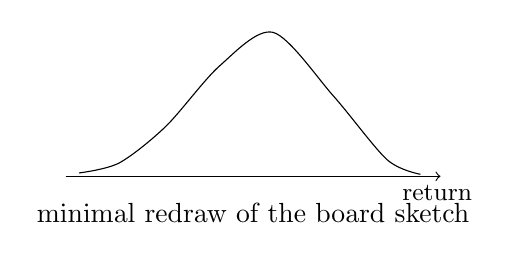
\begin{tikzpicture}[scale=0.85]
\draw[->] (0,0) -- (5.6,0);
\draw[smooth] plot coordinates {(0.2,0.05) (0.8,0.20) (1.5,0.75) (2.3,1.65) (3.1,2.15) (4.0,1.20) (4.8,0.25) (5.3,0.03)};
\node at (2.8,-0.55) {minimal redraw of the board sketch};
\node at (5.55,-0.25) {\small return};
\end{tikzpicture}
\hspace{1cm}
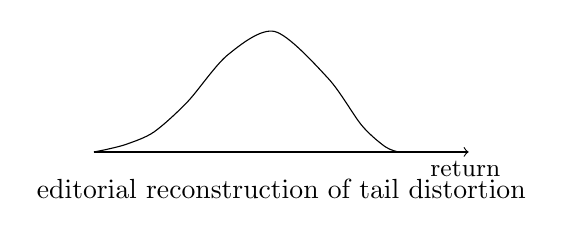
\begin{tikzpicture}[scale=0.85]
\draw[->] (0,0) -- (5.6,0);
\draw[smooth] plot coordinates {(0.0,0.00) (0.2,0.04) (0.5,0.12) (0.9,0.30) (1.4,0.75) (2.0,1.45) (2.7,1.80) (3.5,1.10) (4.0,0.40) (4.35,0.08) (4.55,0.00)};
\node at (2.8,-0.55) {editorial reconstruction of tail distortion};
\node at (5.55,-0.25) {\small return};
\end{tikzpicture}
\caption{Left: a minimal redraw of the bell-shaped return distribution visible on the board. Right: an editorial reconstruction of the lecture's verbal mechanism, with reduced upside tail and deeper downside tail. The asymmetry on the right is transcript-based exposition, not a literal redraw of the frame.}
\end{figure}

\section{Integral Investment Management, disclosure, and the moral of the Swensen recap}

Shiller immediately insists that this is not merely an academic possibility. He cites Integral Investment Management, a hedge fund that used an options strategy of roughly this kind. Investors poured money into it. Most notably, the Art Institute of Chicago placed roughly \$43 million into the fund and related vehicles. When the market fell sharply in 2001, the strategy collapsed and the Art Institute lost almost all of that investment.

The institution had been seduced by what looked like genius. The fund had one of the highest Sharpe ratios in the industry. But the high ratio was not evidence of safety. It was evidence that the measured statistics were concealing the true structure of the payoff distribution.

This leads to a second moral, and in Shiller's hands it becomes broader than finance arithmetic. The law, as he states it, does not permit an investment manager merely to hide behind boilerplate language. If there is relevant information that would make the reported statistics misleading, one must actively disclose it and bring it to the investor's attention. Boilerplate disclaimers of the form ``past returns are not a guide to the future'' do not suffice when the real issue is a specific embedded tail risk.

The lecture then returns to Swensen from a different angle. The essence of Swensen's contribution is not the manipulation of a performance statistic. It has to do with character, reputation, integrity, and institutional purpose. In actual finance careers, clients cannot fully infer what a manager is doing from summary numbers alone. They judge the person, the objective, and the disclosure environment. Only after this detour does Shiller say, in effect: now let us go directly into efficient markets.

\section{Before the phrase: Gibson, Reuters, and Conant}

Shiller's history begins before the phrase ``efficient markets hypothesis'' had become a standard label. The earliest clear formulation he identifies is George Gibson in 1889. Gibson's idea is not dressed up in modern notation, but its content is already recognizable. Once shares are publicly known in an open market, the resulting price may be taken as the judgment of the best intelligence available about them.

This is a voting-machine picture, but not in the trivial sense of counting opinions. If we believe a security is undervalued, we vote by buying it. If we believe it is overvalued, we vote by selling it. Those who are better informed or more capable have both stronger incentives and, after repeated success, more capital with which to vote. The price becomes a social aggregator of intelligence.

A second element in Gibson's account is speed. He writes in what he calls a modern electric age. In 1889 that means telegraphy, ticker machines, and rapid transmission of quotes. The point is already recognizably modern: information moves quickly, and because it moves quickly, profit opportunities based on public information vanish quickly.

\begin{figure}
\centering

\includegraphics[width=0.78\textwidth]{lecture_07_figure_03.png}
\caption{The historical chalkboard layout: George Gibson, Reuters, and Charles Conant. The cropped writing at the far left belongs to an earlier board state and should not be read as part of the historical genealogy.}
\end{figure}

Shiller then gives the history a more concrete institutional edge with Reuters. Before telegraphy dominated, Reuters used carrier pigeons to move financial information between London and Paris. The method is quaint only if we ignore the economics. A trader who receives important news hours before other traders can earn enormous gains. Information speed is therefore not decorative. It is the engine behind the intuition of market efficiency.

The same point appears in Shiller's modernized example of a drug announcement. News arrives. Analysts scramble. Specialists refine their judgments minute by minute. The price jumps, jiggles, and then settles toward a new level within a short interval. By the time a retail investor reads the news the next morning, the opportunity associated with that public announcement is gone. In precisely this sense the hypothesis contains truth: public news is old news with astonishing speed.

Conant, writing in 1904, makes the next move. He begins by attacking the accusation that stock-market speculation is merely gambling. That accusation, he says, cannot be the whole story, because the stock market is a central institution of modern economies. If all the stock exchanges of the world were closed, no one would know what assets were worth, capital would lose its signals, and economic calculation itself would be impaired. Quoted prices do not merely entertain speculators. They help direct investment across industries.

\subsection{Question \& Answer}

Why is a stock market a central economic institution rather than just an organized gambling hall?

Because quoted market prices perform a social function. They summarize information, permit comparison, and guide the movement of capital. Without them, investors and firms are partially blind. Conant's point is not that gambling motives are absent from finance. It is that the market does something far more important than gambling: it produces publicly observed price signals that organize modern economic life.

\section{From doctrine to revision: Roberts, Fama, and CRSP}

The phrase itself emerges later. Shiller credits Harry Roberts at the University of Chicago with the label, and Eugene Fama with making the idea famous. The Chicago setting matters because the theory's rise was inseparable from a new data infrastructure. In 1960 the Ford Foundation funded the assembly of a systematic stock-price database stretching back to 1926, correcting for stock splits, dividends, and similar complications. The institution built for this purpose was the Center for Research in Security Prices, now commonly abbreviated CRSP.

This changed the tone of the debate. Once long price histories were organized and machine-readable, market efficiency could be tested at scale. By the late 1960s thousands of papers were examining the question. Fama's 1969 review article \emph{Efficient Capital Markets} gave the new literature an authoritative summary. His conclusion was not that the evidence was perfectly uniform, but that markets were remarkably efficient. The profession heard something even stronger: perhaps there was simply no way to beat the market except by luck.

In the 1970s this looked like a triumph. Investment managers were implicitly challenged by a theory that seemed to say their success stories were either luck or illusion. Yet Shiller's historical point is that the orthodoxy later softened without disappearing. Older textbooks could still say, with remarkable confidence, that security prices reflect the true underlying value of assets. Later editions stepped back and admitted that prices sometimes stray far from what seems justified by discounted future payoffs.

Shiller uses Jonah Lehrer's phrase ``the truth wears off'' to describe this kind of intellectual reversal. A research program may begin with real insights, become overconfident, and then retreat as anomalies accumulate. That does not mean the original idea was worthless. It means that a useful truth was taken too far. Efficient markets, in this lecture, is exactly such a case.

\section{Technical analysis as the foil}

Only after this historical buildup does Shiller bring in technical analysis. The sequencing matters. Technical analysis is not introduced as a joke. It is introduced as a serious rival intuition. Its practitioners study price charts directly and search for patterns that may reveal future movements. Edwards and McGee are the canonical names, and McGee in particular is presented as someone deeply interested in market psychology.

Two examples organize the discussion. The first is the resistance level. When the Dow first approached 1000, technicians argued that the market might have difficulty crossing so psychologically weighty a number. The claim sounds mystical until one remembers that traders are human beings who may indeed sell at salient round numbers. The second example is the head-and-shoulders pattern: two smaller shoulders around a higher peak, supposedly followed by a collapse.

The important question is not whether such patterns can be drawn after the fact. Of course they can. The question is whether they create robust, tradable profit opportunities.

\subsection{Question \& Answer}

Does technical analysis actually work, or does it only find patterns in noise?

Shiller's answer is carefully intermediate. It is too crude to call all of technical analysis nonsense. He notes that the early efficient-markets literature often dismissed chartist claims more completely than the actual evidence justified. Later work found some element of truth in a few of the classic observations. But the opposite exaggeration is just as wrong. Technical analysis is not a reliable short-run path to riches. At most it is a subtle art that may occasionally augment broader trading judgment.

This prepares the final turn. To decide whether patterns are meaningful, we need a benchmark for what sheer unstructured price movement looks like. That benchmark is the random walk.

\section{Random walk, AR(1), and the half-truth}

If prices are already efficient, then day-to-day changes should be driven by new information. But new information is, by definition, unforecastable. This gives the random-walk intuition. Price changes are not mechanically caused by yesterday's visible chart pattern; they are caused by shocks that were not known yesterday.

\begin{definition}
A random walk is a process \(\{X_t\}\) satisfying
\begin{align}
X_t &= X_{t-1} + \epsilon_t, \\
E[\epsilon_t] &= 0,
\end{align}
where \(\epsilon_t\) is an unforecastable innovation.
\end{definition}

For the blackboard mathematics, Shiller takes the convenient idealization that the shocks have some standard deviation \(\sigma_\epsilon\) and are perhaps even Gaussian:
\begin{equation}
\epsilon_t \sim N(0,\sigma_\epsilon^2).
\end{equation}
He later backs away from taking Gaussianity too seriously, but it is a useful classroom starting point.

The historical image behind the random walk is Carl Pearson's drunk at the lamppost. The drunk has no directional plan. Asked for the best forecast of his position in ten minutes, we do not predict a systematic drift away from the lamppost. We predict the current position, but with growing uncertainty around it.

\begin{proposition}
If the shocks \(\epsilon_t\) are independent with mean zero, then for the random walk
\begin{equation}
E[X_{t+n}\mid X_t] = X_t,
\end{equation}
and the dispersion of the \(n\)-period forecast grows with the square root of horizon:
\begin{equation}
\operatorname{Var}(X_{t+n}-X_t) = n\sigma_\epsilon^2,
\qquad
\operatorname{SD}(X_{t+n}-X_t) = \sqrt{n}\,\sigma_\epsilon.
\end{equation}
\end{proposition}

\begin{proof}
By iterating the update rule,
\[
X_{t+n}-X_t = \epsilon_{t+1} + \epsilon_{t+2} + \cdots + \epsilon_{t+n}.
\]
Taking conditional expectation given \(X_t\), every shock has mean zero, so the sum has mean zero:
\[
E[X_{t+n}-X_t\mid X_t] = 0,
\]
hence \(E[X_{t+n}\mid X_t] = X_t\). Under independence, variances add:
\[
\operatorname{Var}(X_{t+n}-X_t) = \sum_{j=1}^{n} \operatorname{Var}(\epsilon_{t+j}) = n\sigma_\epsilon^2.
\]
Taking square roots gives the square-root rule for forecast uncertainty.
\end{proof}

Shiller then contrasts this with a first-order autoregressive alternative centered at 100. The board equation, cleaned up in standard notation, is
\begin{equation}
X_t = 100 + \rho(X_{t-1}-100) + \epsilon_t,
\qquad
-1 < \rho < 1.
\end{equation}
The right-hand shock symbol on the board is not perfectly legible, but the transcript makes clear that it is the innovation term \(\epsilon_t\).

\begin{figure}
\centering

\includegraphics[width=0.88\textwidth]{lecture_07_figure_05.png}
\caption{The board comparison between random walk and the AR(1) alternative. The visible structure matters here: Pearson and \emph{Nature} 1905 at left, the AR(1) equation and parameter restriction in the center, and the random-walk equation at right.}
\end{figure}

This model is meant to capture mean reversion. The number 100 plays the role of the lamppost. If the process is above 100, it tends to stay above 100 for a while, but its expected deviation shrinks. If it is below 100, the negative deviation also shrinks in magnitude.

\begin{proposition}
For the AR(1) process
\[
X_t = 100 + \rho(X_{t-1}-100) + \epsilon_t,
\]
if \(E[\epsilon_t\mid X_{t-1}] = 0\), then
\begin{equation}
E[X_t-100\mid X_{t-1}] = \rho(X_{t-1}-100).
\end{equation}
In particular, when \(0<\rho<1\), deviations from 100 shrink in conditional expectation.
\end{proposition}

\begin{proof}
Subtract 100 from both sides:
\[
X_t-100 = \rho(X_{t-1}-100) + \epsilon_t.
\]
Now take conditional expectation given \(X_{t-1}\):
\[
E[X_t-100\mid X_{t-1}] = \rho(X_{t-1}-100) + E[\epsilon_t\mid X_{t-1}]
= \rho(X_{t-1}-100).
\]
If \(0<\rho<1\), the expected deviation keeps its sign but is smaller in absolute value.
\end{proof}

\paragraph{Worked example.}
Shiller gives the concrete case \(\rho=\tfrac12\). If the previous period's value was 20 points above the anchor, say \(X_{t-1}=120\), then
\begin{equation}
E[X_t\mid X_{t-1}=120] = 100 + \frac12(120-100) = 110.
\end{equation}
The process remains above 100, but only half as far above. One period later the expected excess over 100 is halved again. This is the sense in which the process is pulled back.

\subsection{Question \& Answer}

Why does \(\rho=1\) turn the AR(1) process into a random walk, and what changes when \(\rho\) is only slightly below 1?

The reduction is immediate:
\begin{align}
X_t &= 100 + \rho(X_{t-1}-100) + \epsilon_t, \\
\rho=1 \quad \Longrightarrow \quad
X_t &= 100 + (X_{t-1}-100) + \epsilon_t \\
&= X_{t-1} + \epsilon_t.
\end{align}
So the special case \(\rho=1\) removes the pull back to the anchor. The lamppost no longer exerts any force. The drunk wanders freely.

If \(\rho\) is only slightly below 1, however, the pull back is extremely weak. This is Shiller's ``loose elastic band'' metaphor. The process is not a pure random walk, because eventually there is reversion. But the reversion may take ten or twenty years to assert itself. In short samples the path may be almost indistinguishable from a random walk. That is why the random-walk idea can contain genuine insight without being exactly right.

The simulation discussion is meant to make this visual. Generated random walks often look surprisingly like the long history of the stock market. A low-\(\rho\) AR(1), by contrast, hugs its trend too closely and creates profit opportunities that look too easy. If prices reliably swung back toward trend over short horizons, one could simply buy below trend and sell above trend. Shiller's point is that the actual stock market does not look like that easy world.

He also corrects himself during the spreadsheet demonstration: some of the simulated paths include an upward deterministic component. One may represent that schematically as
\begin{equation}
X_t = X_{t-1} + c + \epsilon_t,
\end{equation}
rather than a pure zero-drift random walk. The distinction matters, but it does not overturn the main pedagogical point. Whether or not a drift term is added, a low-\(\rho\) mean-reverting process still looks too tightly tied to its trend compared with long stock-market history.

The random-walk story also has an important defect. In the Gaussian simulations, the crash of 1929 does not really appear. The reason is that normally distributed shocks do not generate sufficiently heavy tails:
\begin{equation}
\epsilon_t \sim N(0,\sigma_\epsilon^2)
\qquad \text{has no fat tails.}
\end{equation}
Thus even the random-walk model with normal shocks is only an approximation. It captures the difficulty of extracting reliable chart patterns, but it misses the empirical violence of rare crashes.

This is where the lecture lands. Simple chartist rules are not powerful short-run money machines. In that sense the efficient-markets hypothesis is right. But if the world is closer to a weakly mean-reverting process with \(\rho\) near 1 than to a perfect random walk, then there may still be long-horizon opportunities. The theory is not false in the crude sense. It is incomplete.

\section{Summary}

We began with the puzzle of David Swensen and ended with the random walk. Between those two points Shiller inserted an essential warning: performance statistics can be gamed, especially when tail risk is hidden. Only after making that warning did he reconstruct the efficient-markets idea historically, from Gibson and Reuters to Conant, Roberts, Fama, and the Chicago data revolution. Technical analysis then served as the foil against which random walk could be made mathematically precise.

The final position is intentionally balanced. Public information is absorbed very quickly. Easy short-run profit rules are therefore elusive. But markets are not so perfectly efficient that every deviation from fundamental value is impossible, nor so Gaussian that crashes are well described by textbook noise. Efficient markets is a half-truth, and the intellectual discipline of the lecture lies in seeing exactly which half is true.